\subsection{Searching}

\begin{frame}[fragile]
\frametitle{Searching}

The implementation of different searching algorithms should be based on
the abstract Search class as given in the following diagram:

\begin{figure}[h]
\centering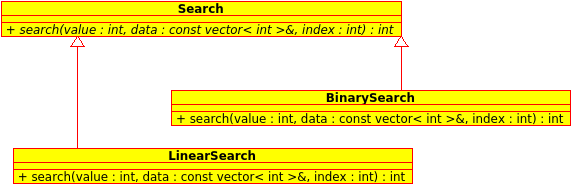
\includegraphics[scale=0.5]{img/search.png}
\caption{Searching Framework}
\end{figure}

\end{frame}

\begin{frame}[fragile]
\frametitle{Searching}
{\tiny
\lstinputlisting{code/search/search.h}
}

\end{frame}

\begin{frame}[fragile]
\frametitle{Linear Search}
Linear search is a method for finding a target value within a list.
It sequentially checks each element of the list for the target value until a match
is found or until all the elements have been searched.\\
\vspace{2mm}
Find 37\\
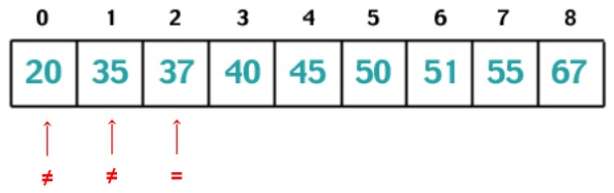
\includegraphics[scale=0.5]{img/linearsearch.png}\\
The result value is 2 (position where 37 is found)\\
\vspace{2mm}
Runtime: $O(n)$
\end{frame}

\begin{frame}[fragile]
\frametitle{Binary Search}
Binary search finds the position of a target value within a sorted array.
It compares the target value to the middle element of the array; if they are unequal,
the half in which the target cannot lie is eliminated and the search continues on the
remaining half until it is successful.\\
\vspace{2mm}
Find 37\\
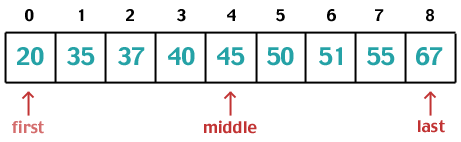
\includegraphics[scale=0.5]{img/binarysearch.png}\\
\vspace{2mm}
Runtime: $O(log(n))$
\end{frame}


